% \begin{table*}[htbp]
% \centering
% \resizebox{.5\linewidth}{!}{\begin{tabular}{lcccc}
% \toprule
% Dataset & \multicolumn{2}{c}{TartanAir v2 Hard} & \multicolumn{2}{c}{TartanAir v2 Easy}\\
%         & $t_{\mathrm{rel}}$ & $r_{\mathrm{rel}}$ & $t_{\mathrm{rel}}$ & $r_{\mathrm{rel}}$\\
% \midrule
% w/o CovKP \& CovOpt  & 0.0916 & 0.5802 & 0.0612 & 0.3918\\
% w/o CovOpt & 0.0795 & 0.4188 & 0.0511 & 0.2766\\
% w/o CovKP  & \underline{0.0186} & \underline{0.1909} & \underline{0.0068} & \underline{0.0771} \\
% \midrule
% \textbf{Ours} & \textbf{0.0171} & \textbf{0.1756} & \textbf{0.0065} & \textbf{0.0723}\\
% \bottomrule
% \end{tabular}}
% \caption{Performance of COVO after partially or fully disabling covariance-related modules.}
% \label{tab: AblationStudy}
% \end{table*}
% \begin{table*}[htbp]
%     \centering
%     \captionsetup{font=small}
%     \begin{minipage}{0.5\textwidth}
%         \centering
%         \caption{Performance of MAC-VO on each ablation setup. Per-trajectory result is shown in \aref{appendix:AdditionalAblation}.}
%         \resizebox{\linewidth}{!}{%
%         \begin{tabular}{lcccc}
%             \toprule
%             Dataset & \multicolumn{2}{c}{TartanAir v2 Hard} & \multicolumn{2}{c}{TartanAir v2 Easy}\\
%                     & $t_{\mathrm{rel}}$ & $r_{\mathrm{rel}}$ & $t_{\mathrm{rel}}$ & $r_{\mathrm{rel}}$\\
%             \midrule
%             w/o CovKP \& CovOpt  & 0.0916 & 0.5802 & 0.0612 & 0.3918\\
%             w/o CovOpt & 0.0795 & 0.4188 & 0.0511 & 0.2766\\
%             % w/o OffDiag
%             w/o CovKP  & \underline{0.0186} & 0.1909 & \underline{0.0068} & 0.0771 \\
%             \midrule
%             DiagCov   & 0.0502 & 0.2991 & 0.0257 & 0.1579 \\
%             FrameNorm & 0.0203 & \underline{0.1780} & 0.0075 & \underline{0.0703} \\
%             PointNorm & 0.0208 & 0.1880 & 0.0077 & 0.0750 \\
%             \midrule
%             \textbf{Ours} & \textbf{0.0138} & \textbf{0.1235} & \textbf{0.0058} & \textbf{0.0611} \\
%             \bottomrule
%         \end{tabular}}
%         \label{tab: AblationStudy}
%     \end{minipage}%
%     \hfill
%     \begin{minipage}{0.48\textwidth}
%         \centering
%         \includegraphics[width=.9\linewidth]{figs/AblationTrajectory.pdf}
%         \vspace{-1mm}
%         \captionof{figure}{\small Results of various ablation setups on the trajectory H05 of TartanAir v2.}
%         \label{fig:AblationSmall}
%     \end{minipage}
%     \vspace{-3mm}
% \end{table*}




\begin{table}[H]
\centering
    \captionsetup{font=small}
    \caption{Ablation study. Detailed results in \aref{appendix:AdditionalAblation}.}
    \resizebox{\linewidth}{!}{
    \begin{tabular}{lcccc}
        \toprule
        Dataset & \multicolumn{2}{c}{TartanAir v2 Hard} & \multicolumn{2}{c}{TartanAir v2 Easy}\\
                & $t_{\mathrm{rel}}$ & $r_{\mathrm{rel}}$ & $t_{\mathrm{rel}}$ & $r_{\mathrm{rel}}$\\
        \midrule
        \textbf{Module Ablation}\\
        \hspace{3mm} w/o CovKP \& CovOpt  & .0743 & .5221 & .0521 & .2799 \\
        \hspace{3mm} w/o CovOpt           & .0679 & .3776 & .0511 & .2367 \\
        \hspace{3mm} w/o CovKP            & \underline{.0188} & .2347 & \underline{.0066} & .0808 \\
        \midrule
        \textbf{Covariance Ablation}      & \\
        \hspace{3mm} DiagCov              & .0461 & .3023 & .0277 & .1548 \\
        \hspace{3mm} Scale Agnostic       & .0204 & \underline{.2321} & .0086 & \underline{.0764} \\
        % \hspace{3mm} Intra-frame Agnostic & 0.0208 & 0.1880 & 0.0077 & 0.0750 \\
        % \yuheng{Diag + Scale Agnostic}\\
        \midrule
        \textbf{Ours}                     & \textbf{.0141} & \textbf{.1429} & \textbf{.0051} & \textbf{.0670}\\
        \bottomrule
    \end{tabular}
    }
    \label{tab: AblationStudy}
    \vspace{-5pt}
\end{table}
\begin{figure}[H]
    \centering
    \captionsetup{font=small}
    \includegraphics[width=.8\linewidth]{tex/ch3_macvo/figs/AblationTrajectory.pdf}
    \caption{Results of various ablation setups on the H01 of TartanAirv2.}
    \label{fig: Ablation}
    \vspace{-5pt}
\end{figure}